\documentclass[tikz,border=2pt]{standalone}
\usepackage{amsmath}
\usepackage{pgfplots}
\pgfplotsset{compat=1.18}

\begin{document}
% A series converges when its partial sums s_n = a_1 + ... + a_n converge: here a_n = 1/2^n,
% s_n = 1 - 1/2^n -> 1.
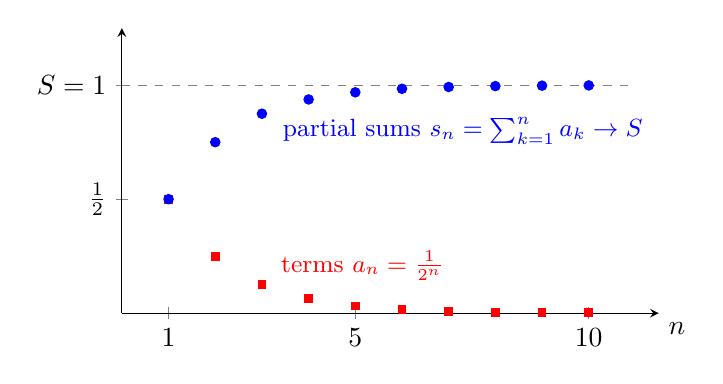
\begin{tikzpicture}
	\begin{axis}[
		axis lines=middle,
		xmin=0, xmax=11.5,
		ymin=0, ymax=1.25,
		xtick={1,5,10}, ytick={0.5,1}, yticklabels={$\tfrac12$,$S=1$},
		xlabel={$n$}, ylabel={},
		xlabel style={below right},
		clip=false,
		width=8.4cm, height=5.2cm
		]
		\addplot[gray, dashed, domain=0:11] {1};
		\addplot[only marks, mark=square*, mark size=1.4pt, red, samples at={1,...,10}] {1/2^x};
		\addplot[only marks, mark=*, mark size=1.7pt, blue, samples at={1,...,10}] {1-1/2^x};
		\node[blue, anchor=north, font=\small] at (axis cs:7.3,0.9) {partial sums $s_n=\sum_{k=1}^{n}a_k\to S$};
		\node[red, anchor=south west, font=\small] at (axis cs:3.2,0.1) {terms $a_n=\tfrac1{2^n}$};
	\end{axis}
\end{tikzpicture}
\end{document}
